\chapter{DESAIN DAN PERANCANGAN}
    Pada bab ini dibahas mengenai analisis dan perancangan sistem.
    
    \section{Deskrisi Umum Sistem}
    	Sistem yang akan dibuat dalam tugas akhir ini adalah sistem yang digunakan untuk melacak perubahan konfigurasi perangkat jaringan. Sistem terhubung dengan perangkat jaringan dan menyimpan semua versi perubahan dari file konfigurasi perangkat jaringan. Sistem bisa mengatur versi konfigurasi yang dibutuhkan oleh perangkat jaringan untuk dipasang pada perangkat jaringan.
    	
    	\indent Sistem memiliki \textit{repository adapter} yang berfungsi untuk menerima file konfigurasi yang dikirim dari perangkat jaringan yang terhubung. Perangkat jaringan mengirimkan file konfigurasi menggunakan protokol pengiriman yang didukung seperti FTP, TFTP, dan SCP. Untuk menyimpan perubahan dari konfigurasi sistem memiliki repositori git untuk menyimpan setiap catatan perubahan yang terjadi pada konfigurasi. Setiap perangkat yang terhubung akan disediakan repositori git untuk masing-masing perangkat. Sistem juga memiliki \textit{repository observer} yang berfungsi untuk melihat setiap perubahan yang terjadi pada konfigurasi perangkat jaringan, setiap ada perubahan maka sistem akan otomatis mencatat perubahan ke dalam repositori git.
    	
    	\indent Di dalam sistem terdapat dua manajemen konsol yang digunakan yaitu Gitea dan Flask. Manajemen konsol tersebut digunakan untuk menerjemahkan instruksi dari administrator kepada sistem sesuai dengan diagram penggunaan pada Gambar \ref{usecase}.
    	
    	\indent Sistem menggunakan basisdata untuk menyimpan data perangkat yang terhubung. Basis data yang digunakan adalah basisdata mysql.
    	
    	\indent Proses penyimpanan konfigurasi dimulai dengan administratur mengirim konfigurasi dari perangkat jaringan menuju sistem. Sistem menerima \textit{file} konfigurasi kemudian mencatat perubahan ke dalam \textit{git repository}. Perubahan disimpan pada \textit{local repository} dan \textit{remote repostory}.
	
    \section{Kasus Penggunaan}
    	Dalam sistem ini hanya ada satu aktor yaitu \textit{administrator} jaringan yang akan mengatur penyimpanan konfigurasi. Terdapat lima fitur utama yang bisa digunakan dalam sistem. Diagram kasus penggunaan sistem pelacakan konfigurasi dapat dilihat pada Gambar \ref{usecase}.
        \begin{figure}[H]
			\centering
			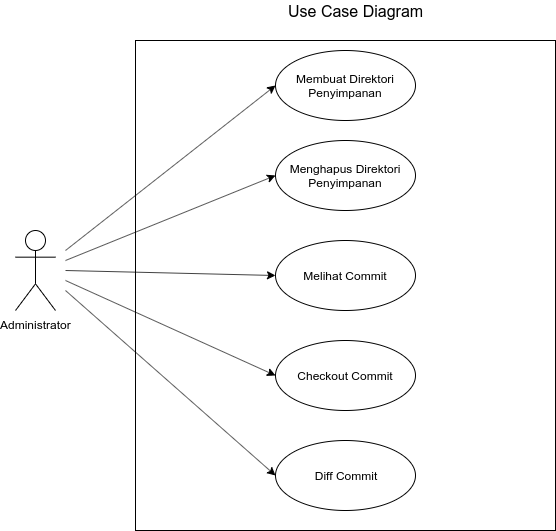
\includegraphics[width=8cm,height=8cm]{Images/C-3/UC-2.png}
			\caption{Diagram kasus penggunaan}
			\label{usecase}
		\end{figure}
        \indent Diagram kasus penggunaan pada Gambar \ref{usecase} dideskripsikan masing-masing pada Tabel \ref {tabelKodeKasusPenggunaan}.
        
        \begin{longtable}{|p{0.25\textwidth}|p{0.24\textwidth}|p{0.35\textwidth}|} % L = Rata kiri untuk setiap kolom, | = garis batas vertikal.
		    	
		    	% Kepala tabel, berulang di setiap halaman
		    
		    	
		    	 \caption{Daftar kode kasus penggunaan} \label{tabelKodeKasusPenggunaan} \\
		    	\hline
		    		\textbf{Kode Kasus Penggunaan} & \textbf{Nama Kasus Penggunaan} & \textbf{Keterangan} \\ \hline
		    	\endfirsthead
		    	\caption[]{Daftar kode kasus penggunaan}   \\
		    	\hline
		    		\textbf{Kode Kasus Penggunaan} & \textbf{Nama Kasus Penggunaan} & \textbf{Keterangan} \\ \hline
		    	\endhead
		    	\endfoot
		    	\endlastfoot
		    	
		    	UC-0001 & Membuat Direktori Penyimpanan. & \textit{Administrator} dapat membuat direktori untuk menyimpan konfigurasi dari perangkat jaringan.\\ \hline
		    	UC-0002 & Menghapus Direktori Penyimpanan.  & \textit{Administrator} dapat menghapus direktori penyimpanan jika sudah tidak digunakan.\\ \hline
		    	UC-0003 & Melihat Commit. & \textit{Administrator} dapat melihat riwayat commit dalam repositori perangkat. \\ \hline
		    	UC-0004 & Checkout Commit. & Administrator dapat berpindah commit (checkout) sesuai dengan versi commit yang diinginkan. \\ \hline
				UC-0005 & Diff Commit. & Administrator dapat melihat perbedaan antara commit satu dengan lainnya. \\ \hline		    	
		    \end{longtable}

	\section{Arsitektur Sistem}
		Pada sub-bab ini, dibahas mengenai tahap analisis dan kebutuhan bisnis dan desain dari sistem yang akan dibangun. Arsitektur sistem secara umum ditunjukkan pada Gambar \ref{DesainUmumSistem}.\\
		\begin{figure}[H]
			\centering
			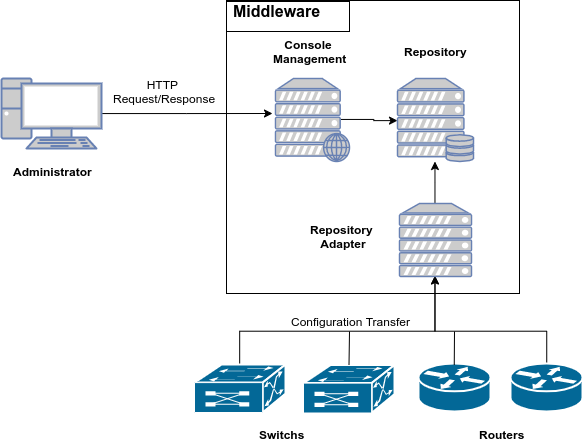
\includegraphics[width=\textwidth]{Images/C-3/Desain-Umum-TA-4.png}
			\caption{Desain umum sistem}
			\label{DesainUmumSistem}
		\end{figure}

		\subsection{Desain Umum Sistem}
			Berdasarkan yang dijelaskan pada deskripsi umum sistem, dapat diperoleh kebutuhan sistem sebagai berikut:
			\begin{enumerate}
				\item \textit{Repository Adapter} untuk menerima konfigurasi yang dikirim dari perangkat jaringan.
				\item Repositori Perangkat untuk menyimpan file konfigurasi dari perangkat jaringan.
				\item \textit{Repository Observer} untuk melihat perubahan file yang disimpan di dalam repository server.
				\item Manajemen Konsol untuk menerjemahkan intruksi dari admin kepada sistem.
			\end{enumerate}
                
                
		\subsection{Perancangan \textit{Repository Adapter} }
			\begin{figure}[H]
				\centering
				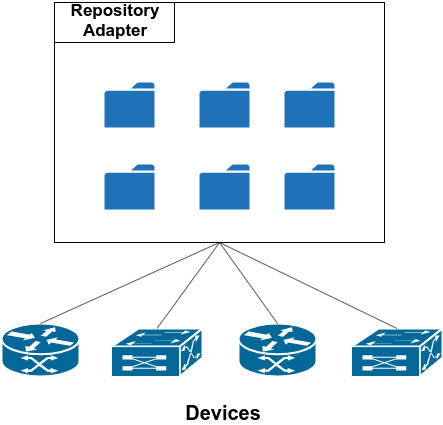
\includegraphics[width=0.9\textwidth]{Images/C-3/Repository-Adapter.png}
				\caption{Desain repositori adapter}
				\label{DesainRepositoriadapter}
			\end{figure}
			\textit{Repository adapter} adalah komponen untuk menerima file konfigurasi yang dikirim dari perangkat jaringan menuju sistem. Sistem dapat menerima pengiriman konfigurasi melalui protokol pengiriman TFTP, FTP, dan SCP. Di dalam \textit{repository adapter} setiap perangkat jaringan yang terhubung memiliki direktori masing-masing. Setiap direktori dikondisikan mampu untuk menerima pengiriman konfigurasi dari \textit{multi-protocol} sehingga perangkat jaringan tidak terbatas satu protokol saja dalam mengirim konfigurasi.\\
			\indent Setelah file konfigurasi diterima oleh \textit{repository adapter} kemudian file konfigurasi dipindahkan ke repositori perangkat. Kemudian di dalam komponen repositori perangkat perubahan file konfigurasi akan dicatat.
			
		\subsection{Perancangan Repositori Perangkat}
		\begin{figure}[H]
			\centering
			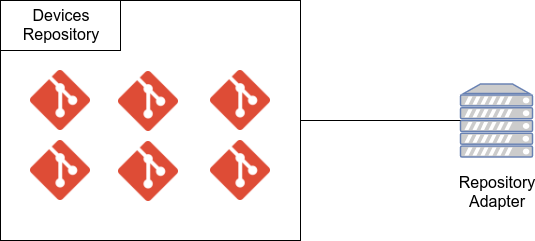
\includegraphics[width=\textwidth]{Images/C-3/devices-repository.png}
			\caption{Desain repositori perangkat}
			\label{DesainRepositoriPerangkat}
		\end{figure}
			Repositori perangkat merupakan komponen untuk mencatat seluruh perubahan yang dilakukan pada file konfigurasi. Repositori perangkat berupa direktori yang berperan sebagai repoitori git. Setiap ada konfigurasi yang dikirim dari perangkat jaringan, konfigurasi akan diterima oleh \textit{repository adapter} kemudian dipindahkan ke dalam repositori perangkat untuk dicatat perubahannya menggunakan git. Di dalam repositori perangkat terdapat dua macam repositori git yakni \textit{local repository} dan \textit{remote repository}. Local repository terhubung dengan manajemen konsol yang berbasis Flask. \textit{Remote repository} terhubung dengan manajemen konsol berbasis gitea. \\
			\indent Di dalam repositori perangkat terdapat terdapat komponen \textit{repository observer} yang melihat perubahan file konfigurasi. Setiap ada file konfigurasi yang dipindahkan dari \textit{repository adapter} maka akan diidentfikasi sebagai perubahan konfigurasi di dalam repositori perangkat.

		
            
        \subsection{Perancangan \textit{Repository Observer}}
            Pada sistem ini \textit{Middleware} harus bisa mengamati repositori perangkat jaringan secara berkelanjutan dan melakukan update pada \textit{history} commit pada repositori. Untuk melakukan hal tersebut modul watchdog di dalam \textit{middleware} yang akan melihat setiap perubahan pada respositori perangkat jaringan. Modul watchdog berjalan sebagai thread yang menunggu perubahan kondisi di dalam repositori. Ketika thread mengidentifikasi ada perubahan di dalam repositori maka thread akan menjalankan perintah commit menggunakan modul gitPython yang terintegrasi dengan middleware. Alur dari repository observer dalam mencatat perubahan dapat dilihat pada gambar\ref{desain_pengirimanfile}.
            \begin{figure}[H]
            	\centering
            	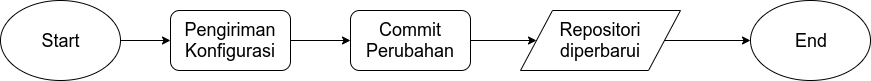
\includegraphics[width=10cm,height=1cm]{Images/C-3/AlurPengirimanFile.png}
            	\caption{Alur pengiriman file}
            	\label{desain_pengirimanfile}
            \end{figure}
        	\indent Salah satu fungsi yang ada dalam sistem adalah fungsi \textit{checkout commit} atau pindah versi konfigurasi. Untuk menjalankan fungsi tersebut \textit{repository observer} harus berhenti sementara waktu hinnga posisi head berubah. Setelah posisi head berubah repository observer dijalankan kembali. Hal ini dilakukan agar proses perpindahan versi tidak dianggap perubahan baru yang menyebabkan ada commit baru pada repository. Alur proses checkout dapat dilihat pada gambar \ref{CheckoutBranch}.
        	 \begin{figure}[H]
        		\centering
        		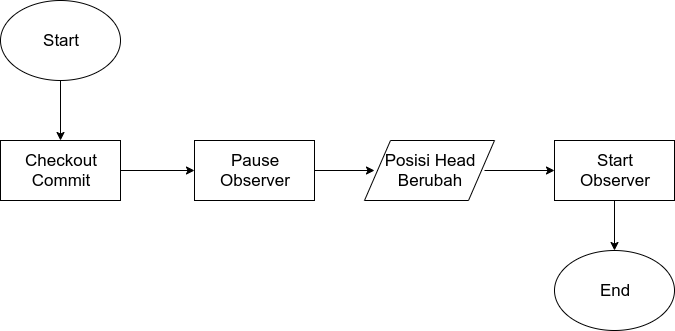
\includegraphics[width=10cm,height=5cm]{Images/C-3/Flow-Checkout.png}
        		\caption{Alur pemindahan versi}
        		\label{CheckoutBranch}
        	\end{figure}
	        \indent Repository Observer juga mengatur pembentukan cabang dari repositori penyimpanan konfigurasi perangkat jaringan. Pembuatan cabang dalam \textit{history} commit diperlukan ketika posisi versi bukan merupakan versi dari perubahan terakhir dalam repositori. Alur pembuatan cabang dari repositori seperti pada gambar \ref{CreateBranch}.
	        \begin{figure}[H]
	        	\centering
	        	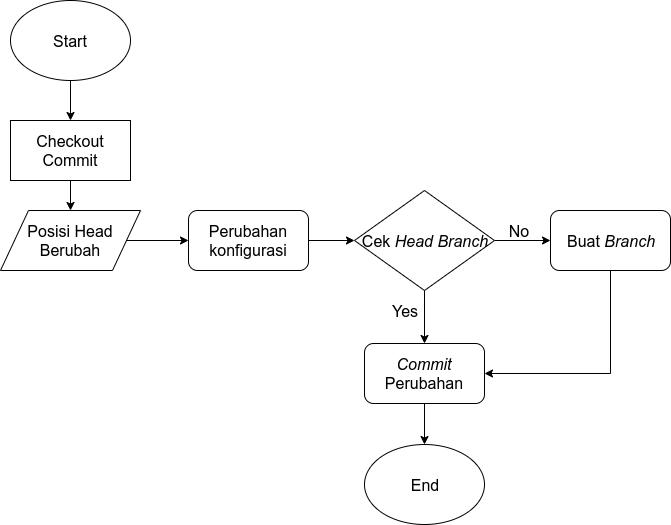
\includegraphics[width=\textwidth]{Images/C-3/CreateBranch.png}
	        	\caption{Alur pembuatan branch}
	        	\label{CreateBranch}
	        \end{figure}
        
        
        \subsection{Perancangan Manajemen Konsol}
        	Dalam sistem yang dibangun, manajemen konsol digunakan untuk menerjemahkan permintaan dari adiministrator jaringan. Manajemen konsol memiliki antarmuka dan rute dengan parameter nama repositori dan permintaan fitur yang diinginkan. Setiap rute akan diproses oleh \textit{Middleware} dan kemudian mengirimkan respon kepada administrator.\\
        	\indent Terdapat dua manajemen konsol yang digunakan dalam sistem pelacakan konfigurasi perangkat jaringan yakni Gitea \textit{webapp} dan Flask. Flask digunakan untuk menampilkan \textit{user interface} dari sistem, akan tetapi flask memiliki keterbatasan dalam fitur melihat isi file konfigurasi dan melihat diff commit atau perbedaan antara commit. Untuk mengatasi permasalahan tersebut maka digunakan Gitea webapp untuk melihat isi file dan perbedaan antara commit.   
         	\begin{figure}[H]
         		\centering
         		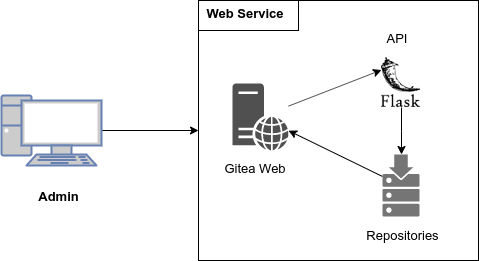
\includegraphics[width=\textwidth]{Images/C-3/Web_Service.png}
         		\caption{Perancangan manajemen konsol}
         		\label{ManajemenKonsol}
         	\end{figure}
         	
         	Desain tampilan web untuk manajemen Konsol dapat dilihat pada gambar\ref{ManajemenKonsolUI}.
         		\begin{figure}[H]
         		\centering
         		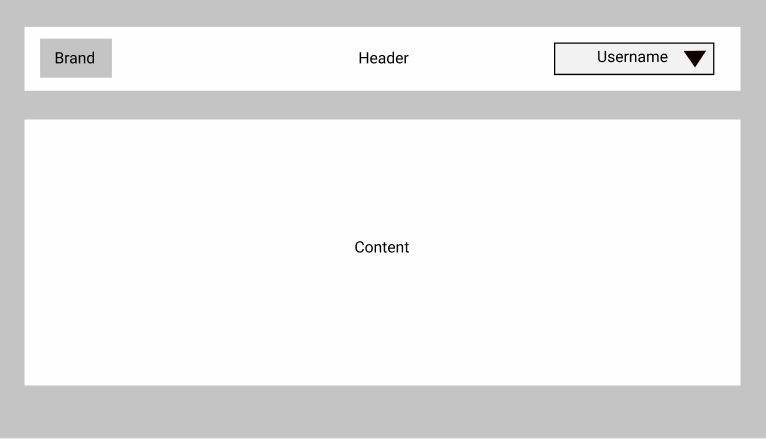
\includegraphics[width=\textwidth]{Images/C-3/desainui.png}
         		\caption{Perancangan tampilan manajemen konsol}
         		\label{ManajemenKonsolUI}
         	\end{figure}
         
         \subsection{Perancangan Basis Data}
         Dalam sistem diperlukan basis data untuk menyimpan data-data yang diperlukan. Basis data digunakan untuk menyimpan data dari perangkat jaringan yang terhubung dengan sistem. Oleh karena itu maka dibutuhkan tabel \textit{device} untuk menyimpan perangkat yang terhubung serta versi konfigurasi yang disimpan. Di dalam basis data data yang disimpan adalah nama perangkat yang terhubung, alamat ip perangkat, serta versi terakhir dari konfigurasi perangkat.
        
       
            
        